\section{Problem Formalization}
\label{sec:formalization}

Real-world text-to-SQL systems often operate in multi-turn interactions, where a user's intent may be underspecified at first and clarified over time. During this process, the intended SQL query may evolve as the user resolves ambiguity or revises a prior choice. We formalize two key interaction patterns:
\textbf{chain ambiguity} and \textbf{user intent drift}.

\subsection{Chain Ambiguity}
\label{subsec:chain} 

\noindent\textbf{Definition.} A sample exhibits \emph{chain ambiguity} when an underspecified user query induces two layers of clarification: \textbf{L1 (layer one)} and \textbf{L2 (layer two)}, such that the existence, scope, or framing of L2 is conditionally dependent on the resolution of L1. Each layer offers two semantically plausible interpretations of the query. This conditional dependency distinguishes \emph{chain ambiguity} from two stacked independent ambiguities, where simply resolving L1 leaves L2's semantic content unaffected.

\namedpara{Counterfactual Test.} To distinguish chain ambiguity from independent stacking, we use the following
\emph{counterfactual test}~\citep{pearl2009causality}: if L1 were resolved with its alternative choice, would L2 still be posed as the same question? The test yields one of three verdicts: (i) \textbf{Eliminated}, where L2's premise vanishes under the L1 alternative and the question becomes vacuous; (ii) \textbf{Transformed}, where L2 must be reframed through changes to its referent, vocabulary, or scope; and (iii) \textbf{Invariant}, where L2 can be asked verbatim, indicating semantic independence. A sample qualifies as chain-ambiguous only when the verdict is \emph{eliminated} or \emph{transformed}; samples judged \emph{invariant} are rejected at this stage.

\namedpara{Worked Example.}
For the dialogue in Figure~\ref{fig:construction}, the L1 alternative
\emph{tenure} measures duration rather than a monetary quantity, so L2's question about excluding refunds no longer has a valid referent. The verdict for this example is therefore \emph{eliminated}.

\begin{figure*}[!t]
  \centering
  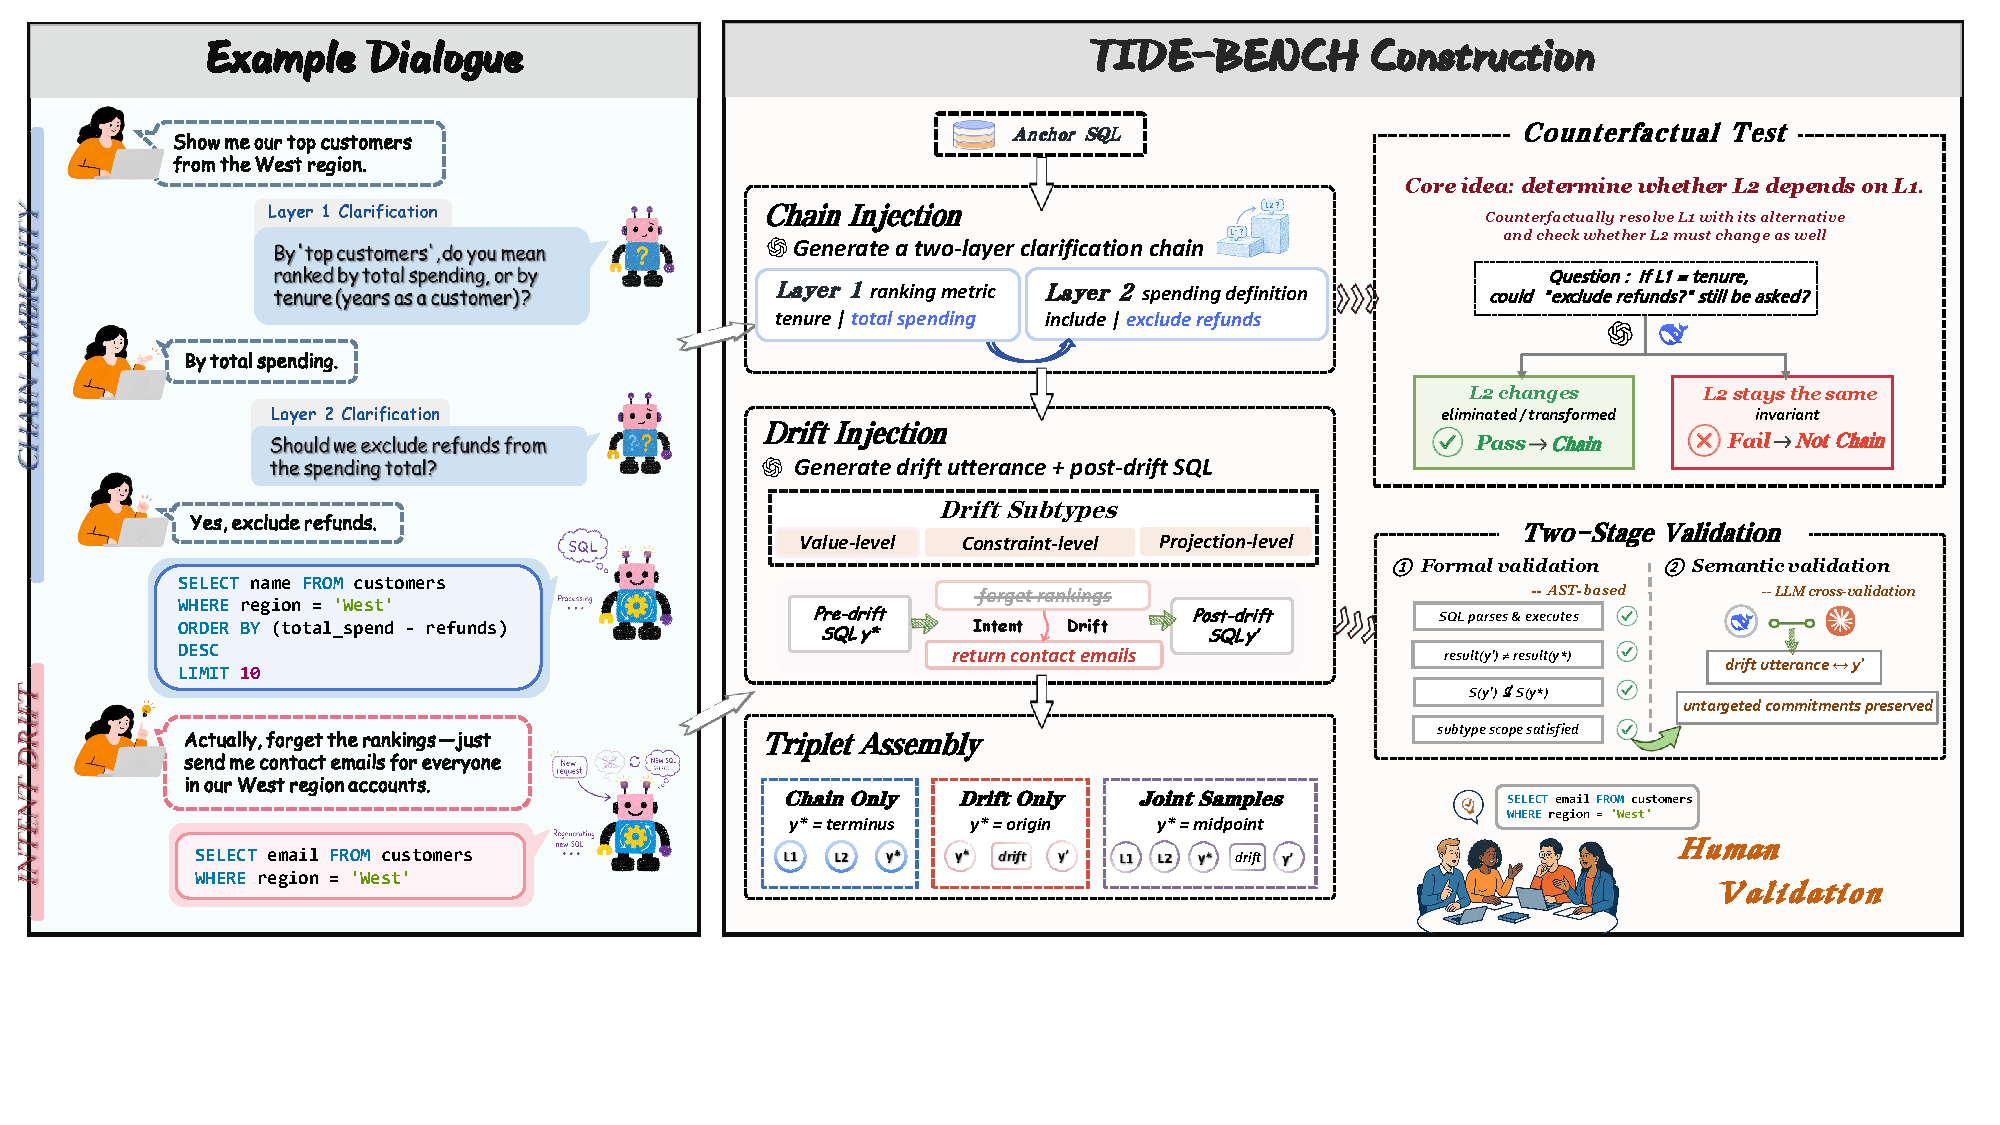
\includegraphics[width=\textwidth]{figure/construction.pdf}
  \vspace{-6mm}
  \caption{\textbf{Left:} motivating dialogue illustrating chain ambiguity (L1/L2 clarification with conditional dependency) and user intent drift (non-monotonic retraction of a prior commitment). \textbf{Right:} overview of the \textsc{TIDE-Bench} four-stage construction pipeline (anchor selection, chain injection, drift injection, and triplet assembly; see \S\ref{sec:construction}).}
  \label{fig:construction}
  \vspace{-4mm}
\end{figure*}

\subsection{User Intent Drift}
\label{subsec:drift}

\noindent\textbf{Definition.}
\emph{User intent drift} is a non-monotonic revision in which at least one previously established commitment is withdrawn or replaced. Unlike cooperative continuation, which retains all prior commitments, drift requires revising the dialogue state and discarding withdrawn requirements from the resulting query but may also introduce new commitments. To formalize this definition, the user's committed intent at each dialogue turn is represented by a SQL query $y$ encoding the intent accumulated up to that turn and a corresponding \emph{commitment set} $S(y)$ directly extracted from its full abstract syntax tree. The set covers filtering predicates, projections, grouping and ordering keys, aggregation filters, and row-limit and offset specifications (Appendix~\ref{app:commitment-extractor}). Let
$S_{\mathrm{pre}}=S(y_{\mathrm{pre}})$ and $S_{\mathrm{post}}=S(y_{\mathrm{post}})$.

\namedpara{Non-Monotonicity Test.}
Drift occurs iff $S_{\mathrm{pre}}\nsubseteq S_{\mathrm{post}}$. The test itself places no restriction on added commitments,
$S_{\mathrm{post}}\setminus S_{\mathrm{pre}}$, and allows removal and replacement while excluding no-change updates and pure additions. Each dialogue contains one controlled drift event, which may affect multiple commitments. This design keeps the pre- and post-drift targets identifiable under the paired design.

\namedpara{Drift Subtypes.}
The benchmark distinguishes three subtypes: (i) \textbf{Value-level}, which replaces only one predicate literal while preserving predicate structure; (ii) \textbf{Constraint-level}, which removes one or more filtering predicates and makes no other uery changes; and (iii) \textbf{Projection-level}, which changes only output-side commitments while preserving all filtering predicates. Algorithm~\ref{alg:drift-test} operationalizes this decision process, first applying the non-monotonicity test and then assigning each accepted drift update to one of the three subtypes.